%  Template for ICASSP-2021 paper; to be used with:
%          spconf.sty  - ICASSP/ICIP LaTeX style file, and
%          IEEEbib.bst - IEEE bibliography style file.
% --------------------------------------------------------------------------
\documentclass{article}
\usepackage{spconf,amsmath,graphicx,hyperref}

% Example definitions.
% --------------------
\def\x{{\mathbf x}}
\def\L{{\cal L}}

% Title.
% ------
\title{AIML 425 Assignemnt 3}
%
% Single address.
% ---------------
\name{Quan Zhao (Student ID: 300471028)}
%\name{Author(s) Name(s)\thanks{Thanks to XYZ agency for funding.}}
\address{Victoria University of Wellington}


\begin{document}
%\ninept
%
\maketitle
%
\section{Introduction}
\label{sec:intro}

body of intro

\{place hold for brief Graph neral netowrk \}

In this work, I will present my understanding of GNN by resolve the "Tiger random walk" problem:

There are 1024 tiger sensors in a square grid in a 3.2 km
by 3.2 km observation area. A tiger enters the area, and then
walks randomly from a sensor to one of eight neighboring
sensors, until it walks out of the area. A fraction $F \in [0, 1]$ of
the sensors does not work. The density of the sensor score s is

\begin{itemize}
  \item $p(s | \text{tiger passed by}) = 1, \quad s \in [0, 1]$
  \item $p(s | \text{no tiger passed by}) = \begin{cases} \frac{2s}{c}, & 0 \leq s < c \\\frac{2(1 - s)}{1 - c}, & c \leq s \leq 1 \end{cases}$
  $\\,\text{(Start with  c = 0 ).}$
\end{itemize}



\section{THEORY}
\label{sec:theory}

\subsection{Graph Convolutional Network (GCN)}
\label{ssec:gcn}

For this problem, a Graph Convolutional Network (GCN) could be a good choice. because:

  \begin{itemize}
    \item Local Neighborhood Information: GCNs are good at aggregating information from a node's local neighborhood, which is crucial for this problem. The tiger's presence at a particular sensor would likely influence the readings of its neighboring sensors.
  
    \item Simplicity and Efficiency: GCNs are relatively simple and computationally efficient compared to some other types of GNNs, making them a good starting point.
  
    \item Node Features: The GCN can easily incorporate node features, which in this case would be the sensor readings.
  
    \item Scalability: GCNs are scalable to large graphs, so if the grid size increases, the model should still perform well.
  \end{itemize}

body of theory \cite{gretton2012kernel}

\section{RESULTS}
\label{sec:results}

To resolve "Tiger random walk" problem. 
The first step is to generate data following the requirements.

In practice, we generate data set by

\begin{enumerate}
  \item A 32 * 32 matrix grid, with $F$ percentage node set as sensor failed.
  \item Tiger's track, by random walk in grid, from edge until reach any other edge.
        \\ Set y label for each node based on the track, if on the track set 1, otherwise set 0.
  \item Update the sensor score $x$ using a probability function of $s$, based on whether the node is on track or not.
\end{enumerate}

The Figure $\ref{fig:data}$ (a) shows a random path the node on track shows red color.
Figure $\ref{fig:data}$ (b) shows scores of nodes, , where larger values correspond to darker colors.

\begin{figure}[htb]
  \begin{minipage}[b]{.48\linewidth}
    \centering
    \centerline{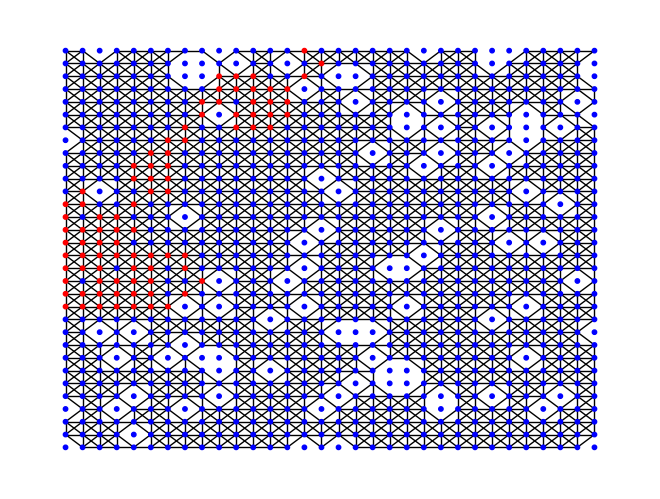
\includegraphics[width=2.5cm]{images/path}}
  %  \vspace{1.5cm}
    \centerline{(a) path of in grid}\medskip
  \end{minipage}
  \hfill
  \begin{minipage}[b]{0.48\linewidth}
    \centering
    \centerline{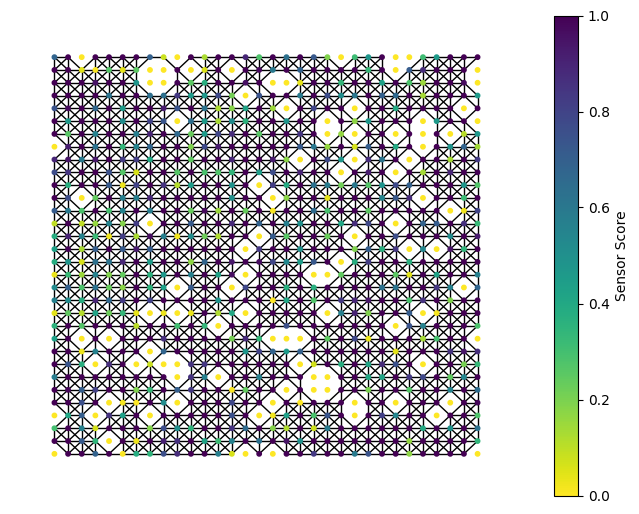
\includegraphics[width=2.5cm]{images/scores}}
  %  \vspace{1.5cm}
    \centerline{(b) node scores in grid }\medskip
  \end{minipage}
  %
  \caption{visulization of dataset}
  \label{fig:data}
  %
  \end{figure}

  In the model training stage, we generate the dataset by following the approach described above. We then split this dataset into training and testing sets.

  We train the model using a 2-layer GCN (Graph Convolutional Network) on the training dataset. The objective function used is Binary Cross-Entropy (BCE) Loss.
  For evaluation, we compute the F1-scores on the test dataset.

  Finally, we measure track accuracy on the test data for various known values of $F$ and $c$.

  The selected values for $F$ are $0, 0.25, 0.75, 1$, and for $c$, the selected values are $1e-09, 0.0017, 0.0032, 0.0056, 1$.
  
  \begin{figure}[htb]

    \begin{minipage}[b]{1.0\linewidth}
      \centering
      \centerline{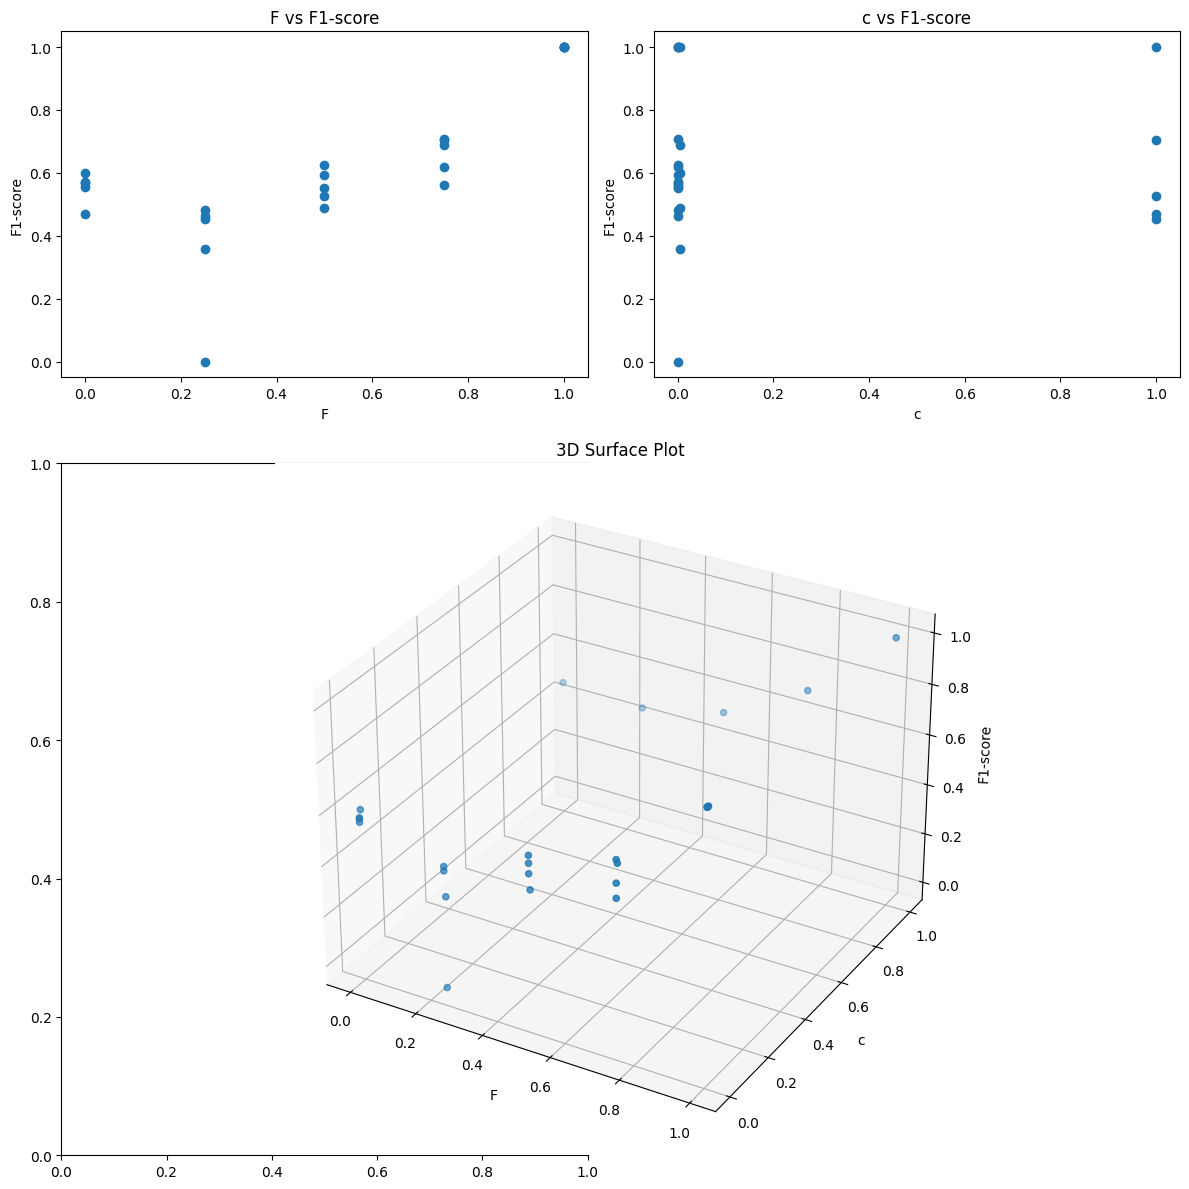
\includegraphics[width=4.0cm]{images/F_c_f1}}
    %  \vspace{2.0cm}
      %\centerline{(a) Result 1}\medskip
    \end{minipage}
    %
    \caption{F1-score distribution with F and c}
    \label{fig:f1}
    %
    \end{figure}


Figure $\ref{fig:f1}$ shows the F1-score value's relationship with F and c score.
Based on the plot results, it appears that the F1-score is affected only when the value of $c$ is close to 0 or 1. For other values of $c$, there seems to be no significant impact on the F1-score.

When $c$ is zero, there is a positive correlation between the F1-score and the value of $F$.
when $c$ is one, the F1-score reaches its lowest point at 
$F$=0.025; beyond that point, both $F$ and the F1-score grow together.

\section{CONCLUSION}
\label{sec:conclusion}

body of conclusion

\section{STATEMENT OF ALL TOOLS USED}
\label{sec:statementofalltoolsused}

body of tools



% To start a new column (but not a new page) and help balance the last-page
% column length use \vfill\pagebreak.
% -------------------------------------------------------------------------
%\vfill
%\pagebreak

\vfill\pagebreak

% References should be produced using the bibtex program from suitable
% BiBTeX files (here: strings, refs, manuals). The IEEEbib.bst bibliography
% style file from IEEE produces unsorted bibliography list.
% -------------------------------------------------------------------------
\bibliographystyle{IEEEbib}
\bibliography{strings,refs}

\end{document}
